\settocdepth{subsubsection}
\chapter{Introduction}
The Simulation Experiment Description Markup Language (SED-ML) is an XML-based format for the description of simulation experiments.

The number of available computational models of biological systems is growing at an ever increasing pace. 
At the same time, their size and complexity are also increasing. The need to build on existing studies by reusing models therefore becomes more imperative. It is now generally accepted that one needs to be able to exchange the biochemical and mathematical structure of models. The efforts to standardise the representation of computational models in various areas of biology, such as the Systems Biology Markup Language (SBML, \citep{Hucka:2003}), CellML \citep{cuellar:2003} or NeuroML \citep{Goddard:2001}, resulted in such an increase of the exchange and re-use of models. 

However, the description of the structure of models is not sufficient for the reproduction of simulation results. One also needs to describe the procedures the models are subjected to, as described by the \emph{Minimum Information About a Simulation Experiment (MIASE)} \citep{Waltemath:2011} which proposes a minimal set of information that should be provided to allow the reproduction of simulation experiments among users and software tools. The increasing use of computational simulation experiments to inform modern biological research creates new challenges to annotate, archive, share and reproduce such experiments. 

SED-ML encodes in a computer-readable exchange format the information required by MIASE to enable reproduction of simulation experiments. It has been developed as a community project and it is defined in this detailed technical specification and in the corresponding XML schema. SED-ML files are encoded in the \emph{Extensible Markup Language} (XML) \citep{Bray:2006} with the format being defined by an XML Schema \citep{Fallside:2001}. 

SED-ML descriptions are independent of the underlying model implementation. SED-ML is a software-independent format for encoding the description of simulation experiments; it is not specific to particular simulation tools.

This document presents \currentLV of the \emph{Simulation Experiment Description Markup Language} (SED-ML), a computer-readable format for encoding simulation experiments. 

\currentLV is the successor of \previousLV and \LoneVone, which is described in \citep{WAB+11}.

\section{SED-ML Content}
A SED-ML document specifies for a given simulation experiment

\begin{itemize}
\item what data to load
\item which models to use in an experiment,
\item modifications to apply on the models before using them,
\item which simulation procedures to run on each model,
\item what analysis results to plot or report,
\item and how these results should be presented
\end{itemize}

SED-ML is build out of the following main objects to describe such information: the \concept{DataDescription}s (added in SED-ML L1V3), the \concept{Model}s, the \concept{Simulation}s, the \concept{Task}s, the \concept{DataGenerator}s, and the \concept{Output}s.

\paragraph{\concept{DataDescription}}

\paragraph{\concept{Model}}
The Model class is used to reference the models used in the simulation experiment. SED-ML itself is independent of the model encoding underlying the models. The only requirement is that the model needs to be referenced by using an unambiguous identifier which allows for finding it, for example using a MIRIAM URI. To specify the language in which the model is encoded, a set of predefined language URNs is provided.

The SED-ML \concept{Change} class allows the application of changes to the referenced models, including changes on the XML attributes, e.g. changing the value of an observable, computing the change of a value using mathematics, or general changes on any XML element of the model representation that is addressable by XPath expressions, e.g. substituting a piece of XML by an updated one.

\paragraph{\concept{Simulation}}
The Simulation class defines the simulation settings and the steps taken during simulation. These include the particular type of simulation and the algorithm used for the execution of the simulation; preferably an unambiguous reference to such an algorithm should be given, using a controlled vocabulary, or ontologies. One example for an ontology of simulation algorithms is the Kinetic Simulation Algorithm Ontology KiSAO. Further information encodable in the Simulation class includes the step size, simulation duration, and other simulation-type dependent information.

\paragraph{\concept{Task}}
SED-ML makes use of the notion of a Task class to combine a defined model (from the Model class) and a defined simulation setting (from the Simulation class). A task always holds one reference each. To refer to a specific model and to a specific simulation, the corresponding IDs are used.

\paragraph{\concept{DataGenerator}}
The raw simulation result sometimes does not correspond to the desired output of the simulation, e.g. one might want to normalise a plot before output, or apply post-processing like mean-value calculation. The DataGenerator class allows for the encoding of such post-processings which need to be applied to the simulation result before output. To define data generators, any addressable variable or parameter of any defined model (from instances of the Model class) may be referenced, and new entities might be specified using MathML definitions.

\paragraph{\concept{Output}}
The Output class defines the output of the simulation, in the sense that it specifies what shall be plotted in the output. To do so, an output type is defined, e.g. 2D-plot, 3D-plot or data table, and the according axes or columns are all assigned to one of the formerly specified instances of the DataGenerator class.

This section provides a high level overview over the content of a SED-ML file. For the detailed technical specification see \hl{??}. 

\section{Motivation: A simulation experiment}
\label{motivation:example}

\hl{TODO MK: add sample experiment to examples in appendix}

The \emph{repressilator} is a rather small, though famous, model that is capable of displaying rich and variable behaviors. We will use this model to demonstrate how a simulation experiment can be described simply and effectively. 

The \emph{repressilator} is a synthetic oscillating network of transcription regulators in Escherichia coli \citep{Elowitz:2000}. The network is composed of the three repressor genes Lactose Operon Repressor (lacI), Tetracycline Repressor (tetR) and Repressor CI (cI), which code for proteins binding to the promoter of the other, blocking their transcription. The three inhibitions together in tandem, form a cyclic negative-feedback loop. To describe the interactions of the molecular species involved in the network, the authors built a simple mathematical model of coupled first-order differential equations. All six molecular species included in the network (three mRNAs, three repressor proteins) participated in creation (transcription/translation) and degradation processes. The model was used to determine the influence of the various parameters on the dynamic behavior of the system. In particular, parameter values were sought which induce stable oscillations in the concentrations of the system components. Oscillations in the levels of the three repressor proteins are obtained by numerical integration. 

\subsection{A time-course simulation}
\label{sec:intro1}
The first experiment we intend to run on the model is the simulation that will lead to the oscillation shown in Figure 1c of the reference publication \citep{Elowitz:2000}. This simulation experiment can be described as:

\begin{enumerate}
 	\item{Import the model identified by the Unified Resource Identifier (URI) \citep{Berners-Lee:2005} \url{urn:miriam:biomodels.db:BIOMD0000000012}.}
 	\item {Select a deterministic method.}
 	\item{Run a uniform time course simulation for 1000~min with an output interval of 1~min.}
 	\item{Plot the amount of \code{lacI}, \code{tetR} and \code{cI} against time in a 2D Plot.}
 \end{enumerate}

Following those steps and performing the simulation in the simulation tool COPASI \citep{Hoops:2006} led to the result shown in \fig{simEx1}. 

\begin{figure}
\centering
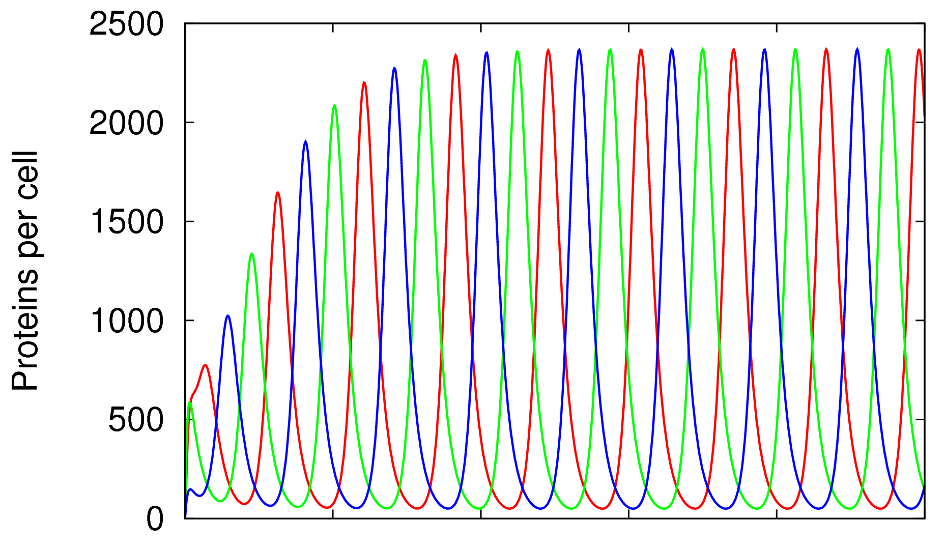
\includegraphics[width=0.6\textwidth]{examples/simEx1.png}
\caption{Time-course simulation of the repressilator model, imported from BioModels Database and simulated in COPASI. The number of repressor proteins lacI, tetR and cI is shown. (taken from \citep{Waltemath:2011})}
\label{fig:simEx1}
\end{figure}

\subsection{Applying pre-processing}
\label{sec:examplePreprocessing}
The fine-tuning of the model can be shown by adjusting parameters before simulation. When changing the initial values of the parameters \emph{protein copies per promoter} and \emph{leakiness in protein copies per promoter} the system's behavior switches from sustained oscillation to asymptotic steady-state. The adjustments leading to that behavior may be described as: 

\begin{enumerate}
\item{Import the model as above.}
\item{Change the value of the parameter \code{tps$\_$repr} from “0.0005” to “1.3e-05”. }
\item{Change the value of the parameter \code{tps$\_$active} from “0.5 “ to “ 0.013“.}
\item{Select a deterministic method.}
\item{Run a uniform time course for the duration of 1000~min with an output interval of 1~min.}
\item Plot the amount of lacI, tetR and cI against time in a 2D Plot.
\end{enumerate}

\fig{simEx3} shows the result of the simulation.

\begin{figure}
\centering
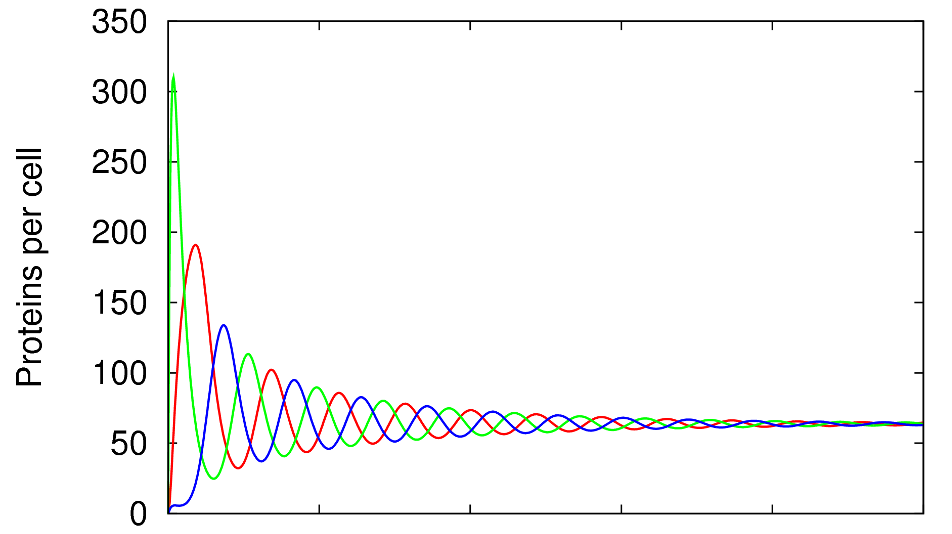
\includegraphics[width=0.7\textwidth]{examples/simEx3.png}
\caption{Time-course simulation of the repressilator model, imported from BioModels Database and simulated in COPASI after modification of the initial values of the \emph{protein copies per promoter} and the \emph{leakiness in protein copies per promoter}. The number of repressor proteins lacI, tetR and cI is shown. (taken from \cite{Waltemath:2011})}
\label{fig:simEx3}
\end{figure}

\subsection{Applying post-processing}
The raw numerical output of the simulation steps may be subjected to data post-processing before plotting or reporting.  In order to describe the production of a normalized plot of the time-course in the first example (section \ref{sec:intro1}), depicting the influence of one variable on another (in phase-planes), one could define the following further steps:

(Please note that the description steps 1 - 4 remain as given in section \ref{sec:intro1} above.)
\begin{enumerate}
\item[5.]{Collect lacI(t) , tetR(t) and cI(t).}
\item[6.]{Compute the highest value for each of the repressor proteins,  max(lacI(t)), max(tetR(t)), max(cI(t)).}
\item[7.]{Normalize the data for each of the repressor proteins by dividing each time point by the maximum value, i.\,e.\ lacI(t)/max(lacI(t) ), tetR(t)/max(tetR(t)) , and cI(t)/max(cI(t)).}
\item[8.]{Plot the normalized \code{lacI} protein as a function of the normalized \code{cI}, the normalized \code{cI}  as a function of the normalized \code{tetR} protein, and the normalized \code{tetR} protein against the normalized \code{lacI} protein in a 2D plot.}
\end{enumerate}

\fig{simEx2} illustrates the result of the simulation after post-processing of the output data. 
\begin{figure}
\centering
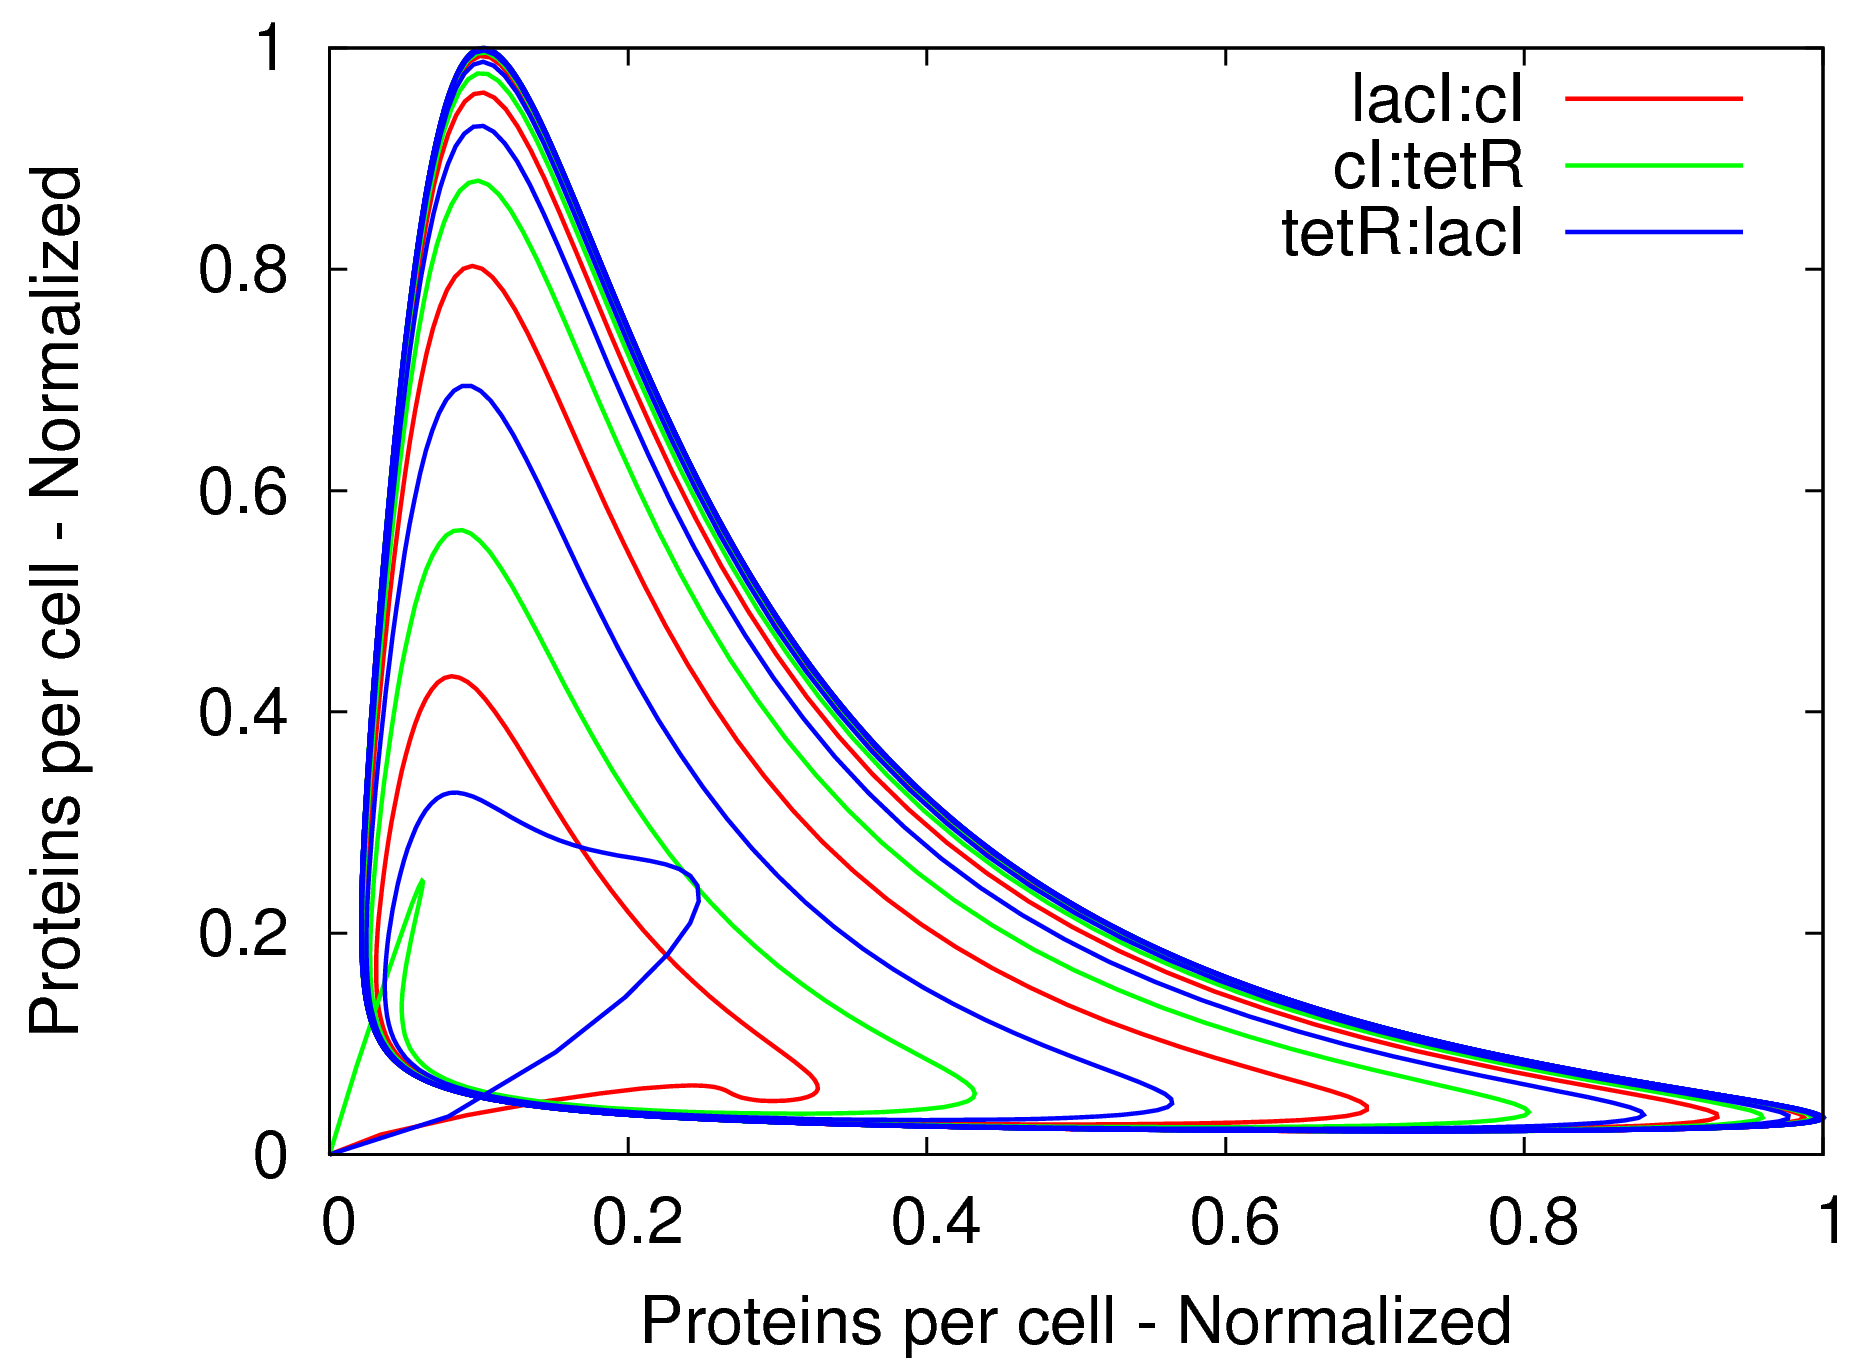
\includegraphics[width=0.7\textwidth]{examples/simEx2.png}
\caption{Time-course simulation of the repressilator model, imported from BioModels Database and simulated in COPASI, showing the normalized temporal evolution of repressor proteins lacI, tetR and cI in phase-plane. (taken from \cite{Waltemath:2011})}
\label{fig:simEx2}
\end{figure}

%%% Local Variables: 
%%% mode: latex
%%% TeX-master: "../sed-ml-L1V3"
%%% End: 
